\documentclass[11pt]{amsart}

\usepackage{geometry}
\usepackage{showlabels}
\usepackage{multirow}
\usepackage{hyperref}
\usepackage{algpseudocode}
\usepackage{todonotes}
\usepackage{algorithm}
\usepackage{enumerate}
\usepackage{graphicx}
%\setlength{\parindent}{0pt}
\geometry{
  includeheadfoot,
  margin=2.54cm
}

\makeatletter
\def\imod#1{\allowbreak\mkern10mu({\operator@font mod}\,\,#1)}
\makeatother

\newtheorem*{problem}{Problem}
\theoremstyle{definition}
\newtheorem*{answer}{Answer}

\newcommand{\R}{\mathbb{R}}
\newcommand{\D}{\mathcal{D}}
\newcommand{\N}{\mathbb{N}}
\newcommand{\Z}{\mathbb{Z}}
\newcommand{\T}{\mathcal{T}}
\newcommand{\C}{\mathcal{C}}
\newcommand{\A}{\mathbb{A}}
\newcommand{\Q}{\mathbb{Q}}
\newcommand{\F}{\mathbb{F}}
\renewcommand{\P}{\mathcal{P}}
\newcommand{\f}{\varphi}
\newcommand{\e}{\epsilon}
\renewcommand{\d}{\delta}

\DeclareMathOperator{\vol}{vol}


\begin{document}

\title{Parallel Conjugate Gradients on sparse stiffness matrices}
\author{Raymond van Veneti\"e \and Jan Westerdiep}
\maketitle

\section{Introduction}
\begin{quote}
``The conjugate gradient method (CG) is an algorithm for the numerical solutions of particular systems of linear equations, namely those whose matrix is symmetric and positive definite. The conjugate gradient method is often implemented as an iterative algorithm, applicable to sparse systems that are too large to be handled by a direct implementation or other direct methods such as the Cholesky decomposition. Large sparse systems often arise when numerically solving partial differential equations or optimization problems." \cite{wiki:cg}
\end{quote}

\begin{quote}
``The finite element method (FEM) is a numerical technique for finding approximate solutions to boundary value problems for partial differential equations. It uses subdivision of a whole problem domain into simpler parts, called finite elements, and variational methods from the calculus of variations to solve the problem by minimizing an associated error function. Analogous to the idea that connecting many tiny straight lines can approximate a larger circle, FEM encompasses methods for connecting many simple element equations over many small subdomains, named finite elements, to approximate a more complex equation over a larger domain." \cite{wiki:fem}
\end{quote}

We will be concerned with solving
\[
  Ax = b
\]
with known $A$ and $b$.

In this report, we will look at a parallel implementation of the conjuate gradient method. We will solve linear systems coming from the finite element method. Systems like this are sparse in the sense that a lot of the elements will be zero. This makes it possible to skip parts of the matrix-vector products one encounters.

To test our implementation, it is useful to have a supply of matrices ready. The University of Florida has a huge collection of sparse matrices. \cite{uniflo} We chose to read these matrices in Matrix Market file format, allowing us to use various tools in existence. \cite{mondriaan,matmar}

\section{Finite Element Method}
Given the boundary value problem, 
\begin{equation}
  \begin{cases} - \Delta u = 1 & \Omega \\ u = 0 & \partial \Omega \end{cases}
  \label{eqn:problem}
\end{equation}
and some partition into simplices, FEM will find the continuous solution, piecewise polynomial (wrt.~this partition) with smallest $H^1$-norm error. ofzo

If we apply this to our 2D case, we have a polygonal domain $\Omega$ and a set of elements $\{\triangle_k\}_{k=1}^K$, $\triangle_k \subset \Omega$ with $\cup_{k=1}^K \triangle_k = \Omega$ and $\triangle_k \cap \triangle_j$ for $k \not= j$ is either empty, a common vertex or a common edge (hoe heet dit ook alweer? regularity condition ofzo?).

We create one reference element $\hat \triangle$ spanned by vertices $(0,0)$, $(1, 0)$, $(0, 1)$ on which we have a polynomial basis of some degree -- say $\bar p$. The amount of basis functions in this basis must be $p = (\bar p + 2)(\bar p + 1)/2$. So we have a basis $\hat \Phi = \{ \hat \phi_i \}_{i=1}^p$.

We are now able to create an affine function $T_k: \triangle_k \to \hat \triangle$ from some element in the partition to this reference element. Hence we automatically have a polynomial basis on $\triangle_k$, namely $\Phi^k := \{ \phi^k_i \}_{i=1}^p$ with $\phi^k_i := \hat \phi_i \circ T_k$.

We can in fact create a global basis $\mathbf \Phi$ by gluing together the correct functions (TODO dit is lastig). Each basis function of this basis is a piecewise polynoimal subject to the partition, and is necessarily zero on $\partial \Omega$.

\subsection{Weak formulation}
If $u$ solves \eqref{eqn:problem}, then
\[
  -\Delta u = 1 \implies - v \Delta u = v \forall v \in H^1_0(\Omega) \implies \int_\Omega - v \Delta u = \int_\Delta v
\]
and using Green's first identity
\[
  \int_\Omega - v \Delta u = \int_\Omega \nabla v \cdot \nabla u - \oint_{\partial \Omega} v( \nabla u \cdot n)
\]
where the last term must equal zero as $u = 0$ on $\partial \Omega$. We therefore end up at the weak formulation:
\[
  u\text{ solves } \eqref{eqn:problem} \implies \int_{\Omega} \nabla v \cdot \nabla u = \int_\Omega v \forall v \in H^1_0(\Omega).
\]

The idea is that we will find functions $u_{FE}$ that exhibit this property and ``hope'' (TODO vinden dat dit klopt) that $u_{FE}$ ``almost'' solves \eqref{eqn:problem}.

\section{Linear polynomials on the triangle}
If we take $\bar p=1$, we are discussing linear polynomials on the triangle. One way to create a basis for this space is to use the \emph{nodal basis}, where we create basis functions that are equal $1$ on one vertex of the triangle and $0$ on the others. The nodal basis on the reference element becomes
\[
  \hat \phi_1 = 1-y-x, \quad \hat \phi_2 = y, \quad \hat \phi_3 = x.
\]

If we look at this globally, we have a \emph{nodal basis} for the whole partition, namely two-dimensional ``hat'' functions $\phi_i$ which are zero on every vertex but a single one -- say $v_i$. The vertices on the boundary of the domain cannot have basis functions associated with them, as the resulting solution $u_{FE} = c^\top \mathbf \Phi = \sum c_i \phi_i$ must be zero on this boundary.

If we fill in $u_{FE}$ in this weak formulation and set $v = \phi_j$, we get
\[
  \int_\Omega \nabla \phi_j \cdot \nabla \left (\sum c_i \phi_i\right) = \int_\Omega \phi_j \implies \sum c_i \int_\Omega \nabla \phi_j \cdot \nabla \phi_i = \int_\Omega \phi_j \forall j
\]
or
\[
  Ac = b, \quad a_{ij} = \int_\Omega \nabla \phi_j \cdot \nabla \phi_i, \quad b_i = \int_\Omega \phi_j.
\]
In other words, finding this best solution $u_{FE} = c^\top \mathbf \Phi$ amounts to solving a linear system where the matrix $A$ is real and symmetric (as inner products are commutative). This is where the Conjugate gradient method comes into play.

Hier moet nog aan toegevoegd worden:
\begin{itemize}
  \item stiffness matrix is eigenlijk som van kleinere stiffness matrices
  \item deze grote stiffness matrix kan je maken/opslaan door op de goede plek shit in te voegen.
\end{itemize}


\section{CG}
In its most basic (sequential, non-preconditioned) form, CG can be written down as in Algorithm~\ref{alg:seqcg}. \cite[Alg.~4.8]{biss04} We slightly adapted it from its original form to be able to use the different BLAS \cite{blas} routines.

\begin{algorithm}
\caption{Sequential CG}
\label{alg:seqcg}
\begin{algorithmic}[1]
  \Require{$k_{max} \in \N$, $\e \in \R$, $n \in \N$, $A$ symmetric $n \times n$, $b \in \R^n$}
  \Ensure{$x \in \R^n$ with $Ax \approx b$}
  \State int $k := 0$;
  \State float $r[n], u[n] = \vec 0, w[n]$;
  \State float $\rho, \rho_{old}, nbsq, \alpha, \beta, \gamma$;
  \State
  \State $r \gets b$;
  \State $\rho \gets \langle r, r \rangle$;
  \State $nbsq \gets \rho$;
  \State
  \While{$\rho > \e^2 \cdot nbsq \wedge k < k_{max}$}
    \If{$k > 0$}
      \State $\beta \gets \rho/\rho_{old}$;
      \State $u \gets \beta u$;\label{line:scaleu}
    \EndIf
    \State
    \State $u \gets r + u$;\label{line:axpyu}
    \State $w \gets Au$;\label{line:mvw}
    \State $\gamma \gets \langle u, w\rangle$;\label{line:ipgamma}
    \State $\alpha \gets \rho/\gamma$;
    \State $x \gets x + \alpha u$;\label{line:axpyx}
    \State $r \gets r - \alpha w$;\label{line:axpyr}
    \State $\rho_{old} \gets \rho$;
    \State $\rho \gets \langle r, r \rangle$;\label{line:iprho}
    \State
    \State $k \gets k+1$;
  \EndWhile
\end{algorithmic}
\end{algorithm}

\subsection{Sparse CG}
As FEM matrices are sparse in nature, we will adapt Algorithm~\ref{alg:seqcg} to a version that supports sparse matrices. For simplicity, we will assume the right-hand side to be dense. This allows us to effectively only change I/O and the function responsible for matrix-vector multiplication.

Our storage format uses the so-called coordinate scheme; we store tuples $(i, j, a_{ij})$ with $i$ the row number, $j$ the column number and $a_{ij}$ the matrix value at this position. The Matrix Market file format adds some headers, e.g. to denounce symmetry so that one only has to store the lower triangular part. We denote by $nz(A)$ the amount of nonzero elements in this lower triangular part. If we store the list of tuples in three lists of length $nz(A)$, namely $I$, $J$ and $v$, we can compute a sequential sparse matrix-vector multiplication using Algorithm~\ref{alg:sparsemv} (from \cite[Alg.~4.3]{biss04}).

\begin{algorithm}
\caption{Sequential sparse matrix vector multiplication: find $y \gets \alpha A x + \beta y$ for symmetric $A$}
\label{alg:sparsemv}
\begin{algorithmic}[1]
  \Require{$\alpha \in \R$, $\beta \in \R$, $n \in \N$, amount of nonzeroes $nz(A)$, $I \in \N^{nz(A)}$, $J \in \N^{nz(Z)}$, $v \in \R^{nz(A)}$, $x \in \R^n$, $y \in \R^n$}
  \Ensure{$y \gets \alpha Ax + \beta y$}
  \For{$i = 0$ until $n$}
    \State $y[i] = \beta y[i]$;
  \EndFor

  \For{$j=0$ until $nz(A)$}
    \State $y[I[j]] = \alpha v[j] x[J[j]] + y[I[j]]$;
    \If{$I[j] \not= J[j]$} \Comment{$A$ is symmetric}
      \State $y[J[j]] = \alpha v[j] x[I[j]] + y[J[j]]$;
    \EndIf
  \EndFor
\end{algorithmic}
\end{algorithm}

\subsection{Preconditioned CG}
The iterates $x_k$ obtained from the CG algorithm satisfy the following inequality \cite[Lect.~7]{sleij}:
\[
  \frac{\|x - x_k\|_A}{\|x - x_0\|_A} \leq 2 \left( \frac{ \sqrt{\kappa_2(A)}-1}{\sqrt{\kappa_2(A)}+1}\right)^k \leq 2 \exp \left( -\frac{2k}{\sqrt{\kappa_2(A)}}\right) 
\]
where $\kappa_2(A)$ is the $2$-condition number of $A$, which for symmetric positive definite matrices equates
\[
  \kappa_2(A) = \frac{\lambda_{max}}{\lambda_{min}}.
\]
It is therefore of interest to create a condition number that is as low as possible.

A preconditioner $P$ of a matrix $A$ is a matrix such that $P^{-1}A$ has a smaller condition number than $A$. As the theoretical convergence rate is highly dependent on the condition number, we can improve this using such a preconditioner. Instead of solving $Ax = b$, we will solve $P^{-1}Ax = P^{-1}b$. This preconditioner should satisy:
\begin{itemize}
  \item Convergence time should be faster for the preconditioned system. Normally, this means that $P$ is constructed as an ``easily invertible'' approximation to $A$;
  \item Operations with $P^{-1}$ should be easy to perform;
  \item $P$ should be (relatively) easy to construct.
\end{itemize}

TODO uitleggen wat implicit preconditioning precies inhoudt

Algorithm~\ref{alg:pcg} shows CG with implicit preconditioning. \cite[Lect.~10]{sleij}
\begin{algorithm}
  \caption{CG with implicit preconditioning \cite[Lect.~10]{sleij}}
  \label{alg:pcg}
  \begin{algorithmic}
    \State $\rho \gets 1$;
    \While{asdf}
      \State $c \gets P^{-1} r$; \Comment{Solve $Pc = r$ for c}
      \State $\rho_{old} \gets \rho$;
      \State $\rho \gets \langle c, r \rangle$;
      \State
      \If{$k > 0$}
        \State $\beta \gets \rho/\rho_{old}$;
        \State $u \gets \beta u$;
      \EndIf
      \State
      \State $u \gets c + u$;
      \State $w \gets Au$;
      \State $\gamma \gets \langle u, w \rangle$;
      \State $\alpha \gets \rho/\gamma$;
      \State $r \gets r - \alpha w$;
      \State $x \gets x + \alpha u$;
    \EndWhile
  \end{algorithmic}
\end{algorithm}

\subsection{Choice of preconditioner}
If $A$ is positive definite, the diagonal tells us a lot about the properties of $A$ so it makes a certain amount of sense to consider perhaps the simplest preconditioner of all:
\[
  P = \text{diag}(a_{11}, \ldots, a_{nn}).
\]
The beauty of this preconditioner is the fact that its sparsity pattern is just like a dense vector. We will use this fact to implement a sparse parallel CG with (rudimentary) preconditioning.

A more advanced preconditioner that is often used in the symmetric positive definite case is Incomplete Cholesky.  The Cholesky factorization of a positive definite matrix $A$ is $A = LL^*$ with $L$ a lower triangular matrix. An incomplete Cholesky factorization is any sparse lower triangular $K$ that is in some sense close to $L$. One such $K$ can be found by finding the exact Cholesky decomposition, except that any entry is set to zero if the corresponding entry in $A$ is also zero. \cite[\S11.5.8]{golub}

\section{Parallellizing CG}
With our sequential algorithm in hand, we are now ready to parallellize the Conjugate gradient method. Given the symmetric positive definite matrix $A \in \R^{n \times n}$ and vector $b \in \R^n$, this requires us to find distributions for $A$, $b$ and all other vectors present in the algorithm. If we want to minimize communication cost, we desire that the distributions of $n, x, r, u, w$ are the same.\footnote{This was also pointed out in \cite[p.~174]{biss04}.} This allows us to perform all vector updates locally and makes for easy implementation of the inner product algorithm.

Every iteration of Algorithm~\ref{alg:seqcg} has 5 vector updates, two inner products and one matrix-vector multiplication. Finding good distributions of $A$, $x$ and $b$ is an NP-hard problem so we will have to resort to heuristic methods. To find these edistributions, we can use Mondriaan.\footnote{Mondriaan is a sequential program written in C that can be used to partition a rectangular sparse matrix, an input vector, and an output vector for parallel sparse matrix-vector multiplication. The program is based on a recursive bipartitioning algorithm that cuts the matrix horizontally and vertically, in a manner resembling some of the famous Mondriaan paintings. The algorithm is multilevel, hypergraph-based, and two-dimensional. It reduces the amount of communication and it spreads both computation and communication evenly over the processors. The program can partition hypergraphs with integer vertex weights and uniform hyperedge costs, but it is primarily intended as a matrix partitioner. \cite{mondriaan}} With its option \texttt{-SquareMatrix\_DistributeVectorsEqual=yes} we can force input and output vector to have the same distribution. We chose not to alter the default load imbalance option of $\epsilon = 0.03$.\footnote{Later inspection using the formula provided in \cite[p.~189]{biss04} -- $\epsilon = Vg/(2nz(A))$ being optimal for the matrix-vector product -- revealed that the optimal value (which of course depends on $p$ and $A$) lies around $0.2$. The total iteration time was however not that much faster, so we opted not to rerun all tests.}

The resulting parallel algorithm is in appearance almost exactly as Algorithm~\ref{alg:seqcg}, so we will not rewrite this. As the vector updates can be done locally without communication, BLAS routines were used (just as in the sequential algorithm). The big changes are made in computation of the inner product and the matrix-vector product. The \texttt{bspmv} algorithm found in \cite[Alg.~4.5]{biss04} was used without alterations, but the \texttt{bspip} algorithm \cite[Alg.~1.1]{biss04} was found unusable as this assumed a cyclical distribution. See Algorithm~\ref{alg:ip} for a parallel inner product algorithm that only assumes that both vectors have the same distribution. The beauty of this algorithm is that no processor has to know the distribution, as long as it has its own vector components stored as a smaller vector.

\begin{algorithm}
  \caption{Parallel inner product $\langle v, y \rangle$ assuming $v$ and $y$ have equal distributions}
  \label{alg:ip}
  \begin{algorithmic}
    \Require{$p$ total number of processors, $0 \leq s < p$ current processor number, $nv_s$ the amount of vector elements locally stored, $v_s,y_s \in \R^{nv_s}$ local vectors}
    \Ensure{$\alpha = \langle v, y \rangle$}
    \State float $\alpha_s = 0$;
    \State float $\alpha = 0$;
    \State 
    \For{$i = 0$ to $nv_s$}\Comment{Compute local inner product}
      \State $\alpha \gets \alpha + v_s[i] \cdot y_s[i]$;
    \EndFor
    \State 
    \For{$q = 0$ to $p$}\Comment{Put local inner product}
      \State Put $\alpha_s$ to $P(q)$;
    \EndFor
    \State 
    \For{$q = 0$ to $p$}\Comment{Find global inner product}
      \State $\alpha \gets \alpha + \alpha_q$;
    \EndFor
  \end{algorithmic}
\end{algorithm}

\subsection{BSP cost}
We first calculate the BSP cost of the parallel algorithm per iteration, using Algorithm~\ref{alg:seqcg} as reference. Let $nv_s$ be the amount of vector elements locally stored on processor $s$. Line~\ref{line:scaleu} costs $nv_s$ operations and lines~\ref{line:axpyu}, \ref{line:axpyx} and \ref{line:axpyr} cost $2nv_s$ each. This makes vector updates contribute $7nv_s$ to the total amount of operations. 

Looking at Algorithm~\ref{alg:ip}, each inner product yields $2nv_s - 1$ operations for Superstep 1, $pg$ operations for Superstep 2 and $p-1$ operations for Superstep 3, with 2 synchronizations in between for a total of $2(2nv_s - 1 + p-1 + pg + 2l)$ inner product operations per iteration.

We found in \cite[p.~189]{biss04} that the matrix-vector product using a Mondriaan distribution yields a total BSP cost of $2(1+\epsilon)nz(A)/p + Vg/p + 4l$ operations. We have one such matrix-vector product per iteration.

Summing everything together, we get a total BSP cost per iteration of
\[
  11nv_s - 4 + p(2+2g) + (Vg + 2 (1+\epsilon)nz(A))/p + 8l.
\]

TODO wat nu? dit relateren aan het aantal iteraties dat nodig is? Wordt snel sketchy

\subsection{Parallel CG with diagonal preconditioner}
TODO

\section{Testing our parallel CG}
To test our implementation, we want to have access to a lot of similar matrices. One way to do this is described in the book: create a random sparse matrix $B$ with values in $[-1,1]$, then take $A \gets B + B^\top + \mu I$ with $\mu$ such that $A$ is strictly diagonally dominant. As the idea of this is merely to generate a matrix $A$ that is symmetric positive definite, we opted for a slightly easier approach. 

We need to compute a \emph{symmetric} matrix, so we only have to look at the lower triangular part of this matrix. First we create a 
random sparse strictly lower triangular matrix $B$. We do this by specifying some
density $\delta$ and placing a random number in $[-1,1]$ on position $(i,j)$ with probability $\delta$. The matrix
must be positive definite, which is achieved \cite[Ex.~24.2]{trefbau} if
\[
  |A_{ii}| > \sum_{j=1, j\ne i}^n |A_{ij}|= \sum_{j=1}^{i-1} |B_{ij}| + |B_{ji}|.
\]
While placing the non-zero entries in the lower triangular part of $B$, we therefore iteratively store the sum in the right hand side of this equation for the
corresponding diagonal element. Let $\mu$ be the maximum of these sums, we now know that $B + B^\top + \mu I$ is a symmetric
positive definite matrix. Finally, to add some more randomness to the diagonal, we replace the diagonal element $\mu$ by a random number in $[\mu, \mu + 2]$ with probability $\delta$.

This parameter $\delta$ gives us an indication for the `sparseness' of the matrix.\footnote{It is actually not the density but the amount of non-zero entries per TODO row/column that is important to the complexity of the matrix-vector product \cite[p.~178]{biss04}. As we are dealing with a square matrix, these two quantities are actually equivalent.} With this method we can generate a variety of matrices
for different combinations of $n$ and $\delta$, which gives insight in the performance of our parallel implementation.

\subsection{Benchmark of Cartesius}
\label{sec:cart}
We ran \texttt{bspbench} with $n=100$, $h=256$ and $p \in \{1, \ldots, 64\}$ to get an idea of values for $r$, $g$ and $l$ for processor counts and get an idea of the scaling properties of Cartesius.

We found the average value of $\bar r = 9157$ Mflop/s. See Figure~\ref{fig:cart} for values of $g$ and $l$ as function of $p$. We see a sharp increase in both $g$ and $l$ at $p=24$ and another one at $p=32$. These have to do with the hardware of Cartesius: under 24 cores is done on a shared-memory system, where communication is cheap. At $p=32$, TODO waarom is dit hoger dan?

\begin{figure}
  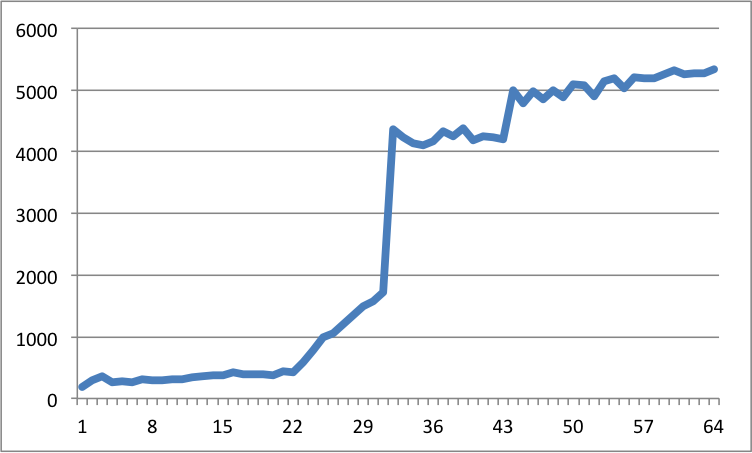
\includegraphics[width=0.49\linewidth]{cartg.png}
  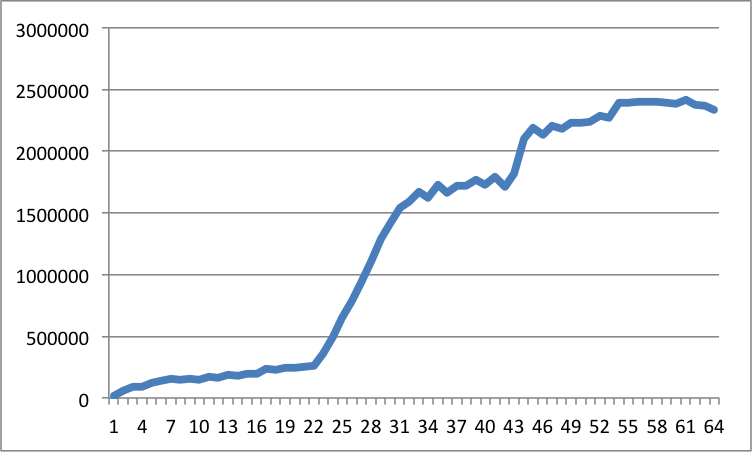
\includegraphics[width=0.49\linewidth]{cartl.png}
  \caption{Results of running \texttt{bsbench} on a thin node of Cartesius with $n=100$, $h=256$. $x$-axis: $p \in \{1, \ldots, 64\}$. $y$-axis: left -- $g$, right -- $l$.}
  \label{fig:cart}
\end{figure}

\subsection{Scaling tests}
With these matrices in hand, we can perform scaling tests by varying 
\[ p \in \{1, 2, 4, \ldots, 64\}, \quad n \in \{64, 128, \ldots, 4096 \}, \quad \delta \in \{0.01, 0.02, 0.03, 0.04, 0.05, 0.1, 0.2\} \]
for slightly less than\footnote{Some matrices created errors. For instance $n = 64, \delta = 0.01$ creates on average $40.96$ non-zeroes. Trying to call Mondriaan with $p=64$ on this matrix generates an error.} $7 \cdot 7 \cdot 7 = 343$ matrices and for each matrix, approximated the solution $x$ to $Ax=b$ with $b$ equal to
\begin{enumerate}
  \item $b = \vec 1 = (1, \ldots, 1)$ (easy right-hand side);
  \item $b = A\vec 1$ (known solution);
  \item $b_i \in [0, 1]$ random (random right-hand side).
\end{enumerate}

For each system, we computed:
\begin{gather*} 
P, n, nz(A), \delta = nz(A)/n^2, k \text{(number of iterations)}, \\
t_i~ \text{(time to initialize)}, \quad t_{mv}~ \text{(time matrix-vector)}, \quad t_{ip}~ \text{(time inner product)}, \\
t_l~ \text{(time local operations)}, \quad t_g~ \text{(time spent computing global solution)}, \\
t_c = t_{mv} + t_{ip} + t_l~ \text{(time spent in while-loop)}, \quad t = t_i + t_{mv} + t_{ip} + t_l + t_g~ \text{(total time)}.
\end{gather*}

The first thing we saw is that the choice of RHS is hardly important for the computation time $t_c$. We therefore made the arbitrary choice to use $b = \vec 1$.

We quickly realized that time spent doing local operations $t_l$ and computing global solution $t_g$ will probably not be of much significance. This was quickly verified: see Figure~\ref{fig:nonsig}.
\begin{figure}
  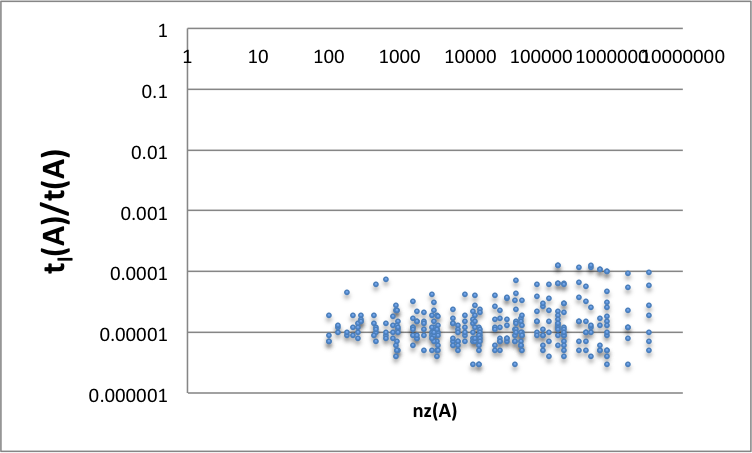
\includegraphics[width=0.49\linewidth]{tlt.png}
  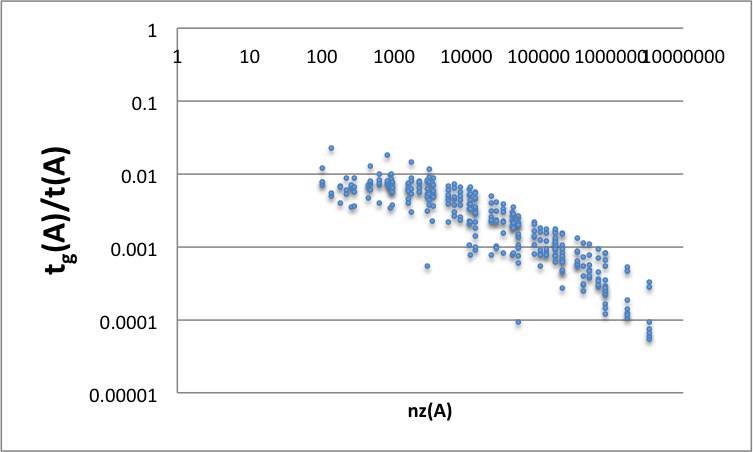
\includegraphics[width=0.49\linewidth]{tgt.png}
  \caption{Percentage of total time spent doing local computations (left) and finding the global solution from the local components (right) for our test matrices.}
  \label{fig:nonsig}
\end{figure}

One other thing we noticed right away is the fact that for our class of matrices $A = B + B^\top + \mu I$, $k$ is very low (in the order of 10). This has the effect that $t_i$ greatly overshadows $t_c$ for large $nz(A)$: see Figure~\ref{fig:quotient}. The reason for this is very insightful to the problem: while strict diagonal dominance implies positive definiteness, it also implies that the diagonal elements are \emph{much} larger than the off-diagonal elements. The resulting matrix is close to being diagonal! As solving $Ax=b$ for a diagonal matrix using CG completes in one step, it is no surprise that CG ends quickly when $A$ is near-diagonal.

\begin{figure}
  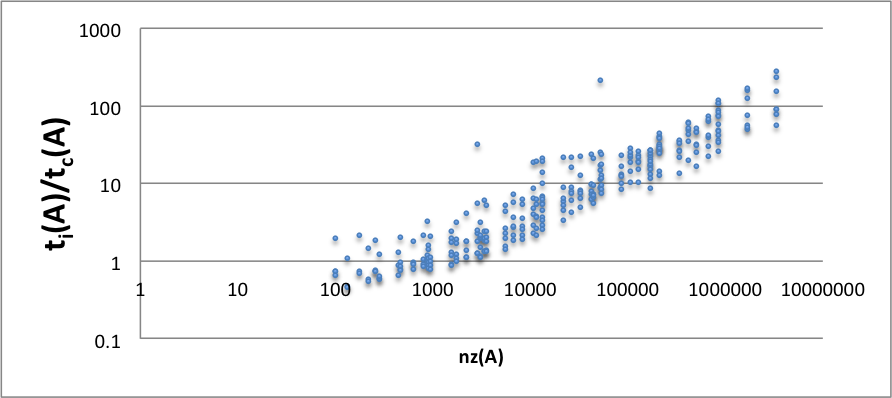
\includegraphics[width=\linewidth]{quotient.png}
  \caption{Quotient of initialization time $t_i$ and computation time $t_c$ for random matrices $A$ as function of $nz(A)$.}
  \label{fig:quotient}
\end{figure}

Taking $n \in \{2048, 4096\}$ and $\delta \in \{0.1, 0.2\}$, we get a few sample matrices. Looking at $t_{mv}$ and $t_{ip}$ for these four matrices yields Figure~\ref{fig:samples}. We see that the optimal computation time ($t_c = t_l + t_{mv} + t_{ip} \approx t_{mv} + t_{ip}$ as $t_l \approx 0$ by Figure~\ref{fig:nonsig}) seems to lie somewhere between $p=8$ and $p=32$. The most likely option is around $p=24$, as this is the highest amount of processor cores that is still on one shared-memory system (see \S \ref{sec:cart}). We can overcome this by increasing the computational effort every processor has to do (increasing $n$ and $nz(A)$), but this proved hard, as Mondriaan takes quite some time to generate the distributions already.

If we look at $t_{mv}$ and $t_{ip}$ separately, we see that for $p=1$, $t_{mv}$ scales linearly with $nz(A)$ (as we concluded before). We also see that for $p=64$, $t_{ip}$ is almost the same across the different matrices. This indicates that the time spent computing the local inner product is heavily outweighed by the communication costs. This raises the question if $t_{ip}$ would improve had we used the inner product communication strategy from the first homework exercise. \cite{TODOHUISWERK} In this exercise, we found that if
\[
  (p - 5\log_2 p) + (p + \log_2 p - 1)g + (2-\log_2 p)l > 0
\]
the new strategy is better. A quick inspection yields that this is true for $p \leq 4$ and \emph{very} false (values being in the order of negative millions), indicating that we won't have to try.

\begin{figure}
  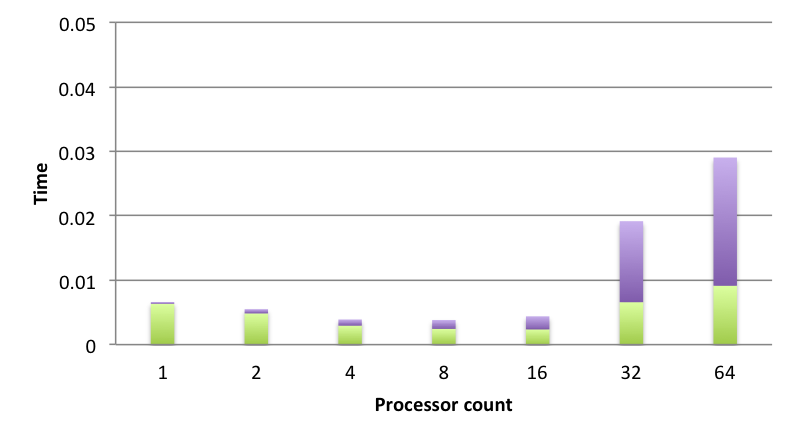
\includegraphics[width=0.48\linewidth]{n2048d0_1mvip.png}
  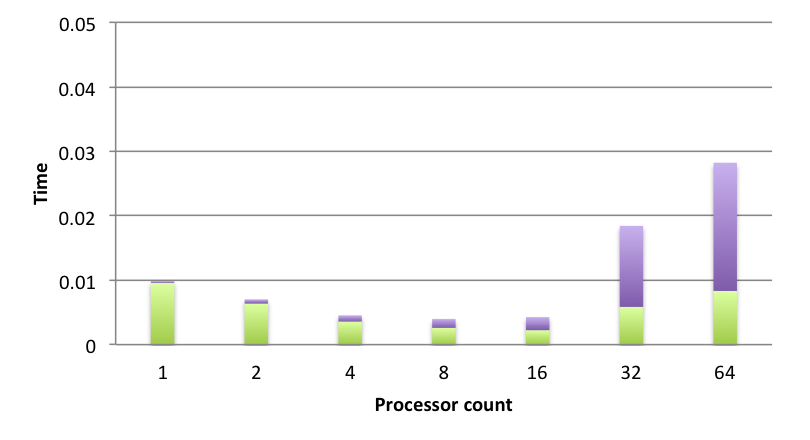
\includegraphics[width=0.48\linewidth]{n2048d0_2mvip.png}
  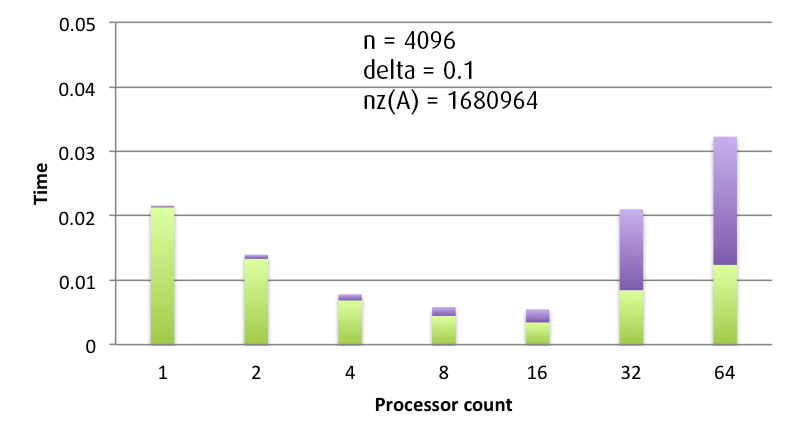
\includegraphics[width=0.48\linewidth]{n4096d0_1mvip.png}
  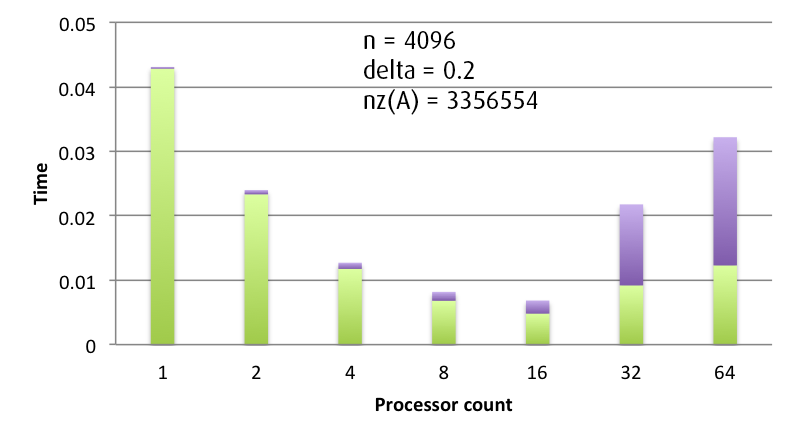
\includegraphics[width=0.48\linewidth]{n4096d0_2mvip.png}
  \caption{Timing results for various sample matrices. Purple: $t_{ip}$; green: $t_{mv}$. Top row: $\delta = 0.1$. Bottom row: $\delta = 0.2$. Left column: $n = 2048$. Right column: $n = 4096$.}
  \label{fig:samples}
\end{figure}

\section{Creating FEM matrices}
\section{hoe heette het ook alweer als je na een kleine verandering in je matrix opnieuw ging optimizen}

\section{Future work}
\subsection{Adaptive FEM}


\bibliographystyle{alpha}
\bibliography{report}

\end{document}
